\subsection{Exponentialfunktion (o-Notation)}
\begin{align*}
    n^l &= o(\exp(n)) \text{ für alle } l > 0\\
    \exp(n) &= e^n = \sum_{j = 0}^{\infty} \frac{n^j}{j!} \text{ wobei } j! = 1 \cdot \dots \cdot (j-1) \cdot j = \Pi_{i = 1}^j i\\
    0! &= 1
\end{align*} 
Wähle $k \in \N$, $k > l$ Dann:
\begin{align*}
    \frac{n^l}{\exp(n)} &= \frac{n^l}{\sum_{j = 0}^{\infty} \frac{n^j}{j!}}\\
    &\leq \frac{n^l}{\frac{n^k}{k!}}\\
    &= \frac{n^l(k!)}{n^k}\\
    &= k! \cdot n^{\overbrace{l - k}^{< 0}}\\
    &= \frac{k!}{n^{k - l}} \hspace{2em} n \rightarrow \infty, \rightarrow 0
\end{align*}
\begin{align*}
    f(n) &= o(y(n)) \text{ falls } \lim_{n \rightarrow \infty} \frac{f(n)}{g(n)} = 0\\
    \rightarrow n^l &= o(\exp(n))
\end{align*}
Allgemeiner:
\begin{align*}
    \forall l > 0, c > 1\\
    n^l = o(c^n)
\end{align*}
Logarithmieren:
\begin{align*}
    \log &= \ln\\
    \log x &= \int_{1}^x \frac{1}{z} dz\\
    \log n &= o(n^\alpha) \text{ für jedes } \alpha > 0
\end{align*}




\subsection{Rechnen mit o(g(n)) und O(g(n))}
$2^{O(n)}$ heißt $2^{f(n)}$ für irgendeine Funktion $f(n) = O(n)$

\begin{align*}
    f(n) &= \frac{1}{n} = O(1)\\
    f(n) &= 10 + \sin(\frac{1}{n}) = \Theta(1)\\
    f(n) &= o(1) \rightarrow f(n) = O(1)\\
    f(n) &= n = \Omega(1)\\
    f(n) &= \sin(n^2) \rightarrow \text{ erfüllt nicht } o(1), \Omega(1), \Theta(1)
\end{align*}

\begin{align*}
    f(n) \sim g(n) \text{ heißt } \frac{f(n)}{g(n)} \rightarrow_{n \rightarrow n} 1
\end{align*}
Beispiel:
\begin{align*}
    f(n) &= n^2 - 10n + 100 \log n\\
    g(n) &= n^2\\
    \frac{f(n)}{g(n)} &= 1 - \overbrace{\frac{10}{n}}^{\rightarrow 0} + \overbrace{\frac{100 \log n}{n^2}}^{\rightarrow 0} \rightarrow_{n \rightarrow \infty} 1
\end{align*}


\subsection{Quicksort-Algorithmus}
Worst-Case: $\frac{n(n+1)}{2}$

\subsection{Permutation erklärt}
\begin{center}
    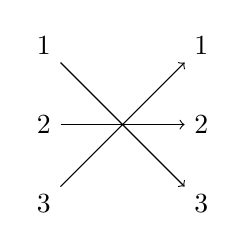
\begin{tikzpicture}
    \node (1) at (0,0) {1};
    \node (2) at (0,-1) {2};
    \node (3) at (0,-2) {3};
    \node (4) at (2,0) {1};
    \node (5) at (2,-1) {2};
    \node (6) at (2,-2) {3};
    \draw[->] (1) to (6);
    \draw[->] (2) to (5);
    \draw[->] (3) to (4);
    \end{tikzpicture}
\end{center}

\subsection{Beweis der Laufzeit vom randomisierten Quicksort}
$X_n =$ erwartete \# Vergleiche auf einer zufälligen $n$-Permutation\\
Es gilt:
\begin{align*}
    X_n &= \overbrace{n}^{\text{Vrgl. mit Pivot}} + \frac{1}{n} \sum_{k =1}^{n} (X_{k-1} + X_{n-k}) & X_1&=1 &X_0 &= 0
\end{align*}

\begin{tabular}{|c|cc|}
     \hline
     k & \dots & \dots\\\hline
\end{tabular}

\begin{align*}
    n \cdot X_n &= n^2 + \sum_{k=1}^{n}(X_{k-1} + X_{n-k})\\
    &= n^2 + 2 \cdot \sum_{k =0}^{n-1} X_k\\
    n+1) X_{n+1} &= (n+1)^2 + 2 \cdot \sum_{k=0}^n  X_k
\end{align*}
\begin{align*}
    (n+1)X_{n+1} - n \cdot X_n = (n+1)^2 - n^2 +2 X_n\\
    &= 2n +1 + 2X_n\\
    (n+1)X_{n+1} &= 2n + 1 + (n+2) X_n
\end{align*}
\begin{align*}
    \frac{X_{n+1}}{n+2} &= \frac{2n+1}{(n+1)(n+2)} + \frac{X_n}{n+1}\\
    &\leq \frac{2}{n+2} + \frac{X_n}{n+1}
\end{align*}

\begin{align*}
    \frac{X_{n+1}}{n+2} &\leq \frac{2}{n+2} + \frac{X_n}{n+1}\\
    &\leq \frac{2}{n+2} + \frac{2}{n+1} + \frac{X_{n-1}}{n}\\
    &\leq \sum_{k=0}^{n +1} \frac{2}{k+1} + \underbrace{\frac{X_0}{1}}_{=0} = 2 H_{n+1}\\
    &\Rightarrow X_{n+1} \leq 2(n+2) H_{n+1} \: \forall n = 2 H_{n+1}
\end{align*}

\begin{align*}
    H_n &\geq \log(n)\\
    &\geq H_n -1\\
    H_n &= \log(n) + O(1)
\end{align*}

\underline{Quicksort:}
\begin{align*}
    2(n+1) H_n = 2(n+1) \log(n) + O(n) \sim 2n\log(n) = \underline{\underline{O(n\log n)}}
\end{align*}